\section{Analysis of filter parallelizability}
Since the filters specify what the processing program should do to each row in a dataset, ``row by row'' or possibly chunks of rows is a suitable
granularity when implementing the parallelization of the program. Consequently, the filters of a file format are the prime candidates
for parallelization analysis. The analysis made is similar to the methodology used to identify the span in the work-span model described in
section \ref{work-span}. When applying the model to the problem of analyzing filters, a task is the processing of one row. In order to find
the tasks that need to be completed before other tasks, the filters that result in state that is accessed by subsequent rows or otherwise
affect the total processing of the dataset need to be identified.

Examining the filters, it is apparent that \textit{Dataset translation}, \textit{Null translation}, \textit{Relation currency},
\textit{Third party automapper}, \textit{Set value}, \textit{RegExp extract}, and \textit{RegExp replace} only operate on the current dataset row, with no side effects.
This means that they produce no state changes that affect subsequent rows, which means that they do not affect the parallelizability of a dataset.

Additionally, \textit{Dataset information}, \textit{Tradefile information}, \textit{Temporary variable}, \textit{Logger}, and \textit{Skip row} perform
operations that either pull information from resources that are available to all rows, or produce an effect that does not affect any other rows.
The \textit{Conditional block} filter only produces effects according to its subfilters (a set of the filters already mentioned), and does not affect parallelization by itself.
\\\\
Hence, the filters that can affect the parallelization of a dataset are:
\begin{itemize}
  \item \textit{Mapping}, since the trade id mapping may need to keep track of state that can be accessed in subsequent rows in order to make all id:s unique.
  \item \textit{Header detection}, since all rows beneath the (first) header row depend on the column names for mappings and other values.
  \item \textit{Global variable}, since the variable may be written and accessed by any subsequent rows. Each rewrite of the variable needs to happen before the next rewrite,
    in the original, sequential order if the verification result is to be correct.
  \item \textit{State variable}, for the same reasons as Global variable.
  \item \textit{Stop processing}, if one thread sees a conditional fulfilled and stops processing, it is possible for another thread to keep processing rows that are intended
    to be ignored, thereby violating the constraints.
\end{itemize}


\section{Code inspection}
After an initial code and file format inspection, the following conclusions where made:
\begin{itemize}
  \item The \textit{Header detection} filter is effectively performed only once, as it is ignored for all rows after the one where the header was found.
  \item The filters \textit{Global variable} and \textit{State variable} make the processing of every row depend on the previous, as the writing of the variables may happen on each row.
  \item The process of making an ID unique could possibly be broken out to a post processing step.
  \item All file formats contain \textit{Header detection}, and many contain the make unique feature of the trade ID mapping.
  \item There are many file formats that do not have either \textit{Global variable}, \textit{State variable} or \textit{Stop processing} among their filters.
\end{itemize}

The conclusions above indicate that header detection may be done before creating the parallel processes, sending this data to each process when they are created.
If the process of producing unique ID:s is then done as a post processing step, the following task DAGs illustrate how the dependencies when processing different
file formats appear: In figure \ref{fig:embarrassing_dag}, the task DAG for a file format without a Global variable or State variable filter is illustrated.
In figure \ref{fig:embarrassing_dag}, the task DAG for a file format containing a Global variable is illustrated. Since the span is equal to the work
in the file formats containing Global variables or State variables, parallelization of datasets with these formats will result in no speedup according to the %Illustrate work-span?
work-span model (as $T_1 \leq T_\infty \Rightarrow S \leq 1$). File formats containing \textit{Stop processing} make it unfeasible to produce correct verification results
when parallelizing. Determination of whether the result is correct is non-viable if any rows are processed in different processes (as rows that should not be included in the result may be included anyway).

\begin{sidewaysfigure}[ht]
  \centering
  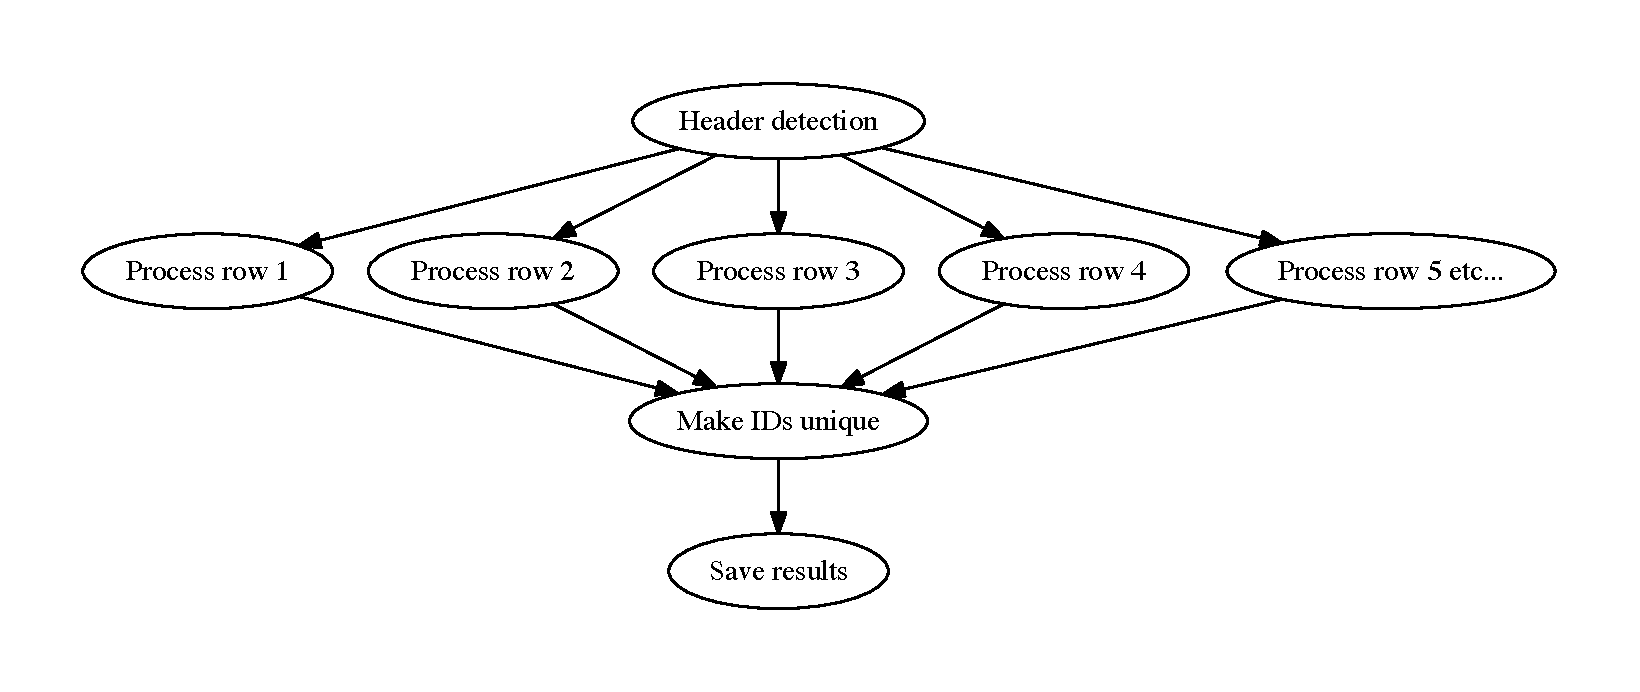
\includegraphics[width=200mm]{figures/embarrassing_file_format.pdf}
  \caption[Task DAG for a file format that does not contain global or state variables.]{An example of a task DAG for a file format that does not contain global variable or state variables. Header detections needs
  to be performed up front, and making trade IDs unique needs to be performed in a post processing step. The processing of each row does not depend on each other.}
  \label{fig:embarrassing_dag}
\end{sidewaysfigure}

\begin{figure}[ht]
  \centering
  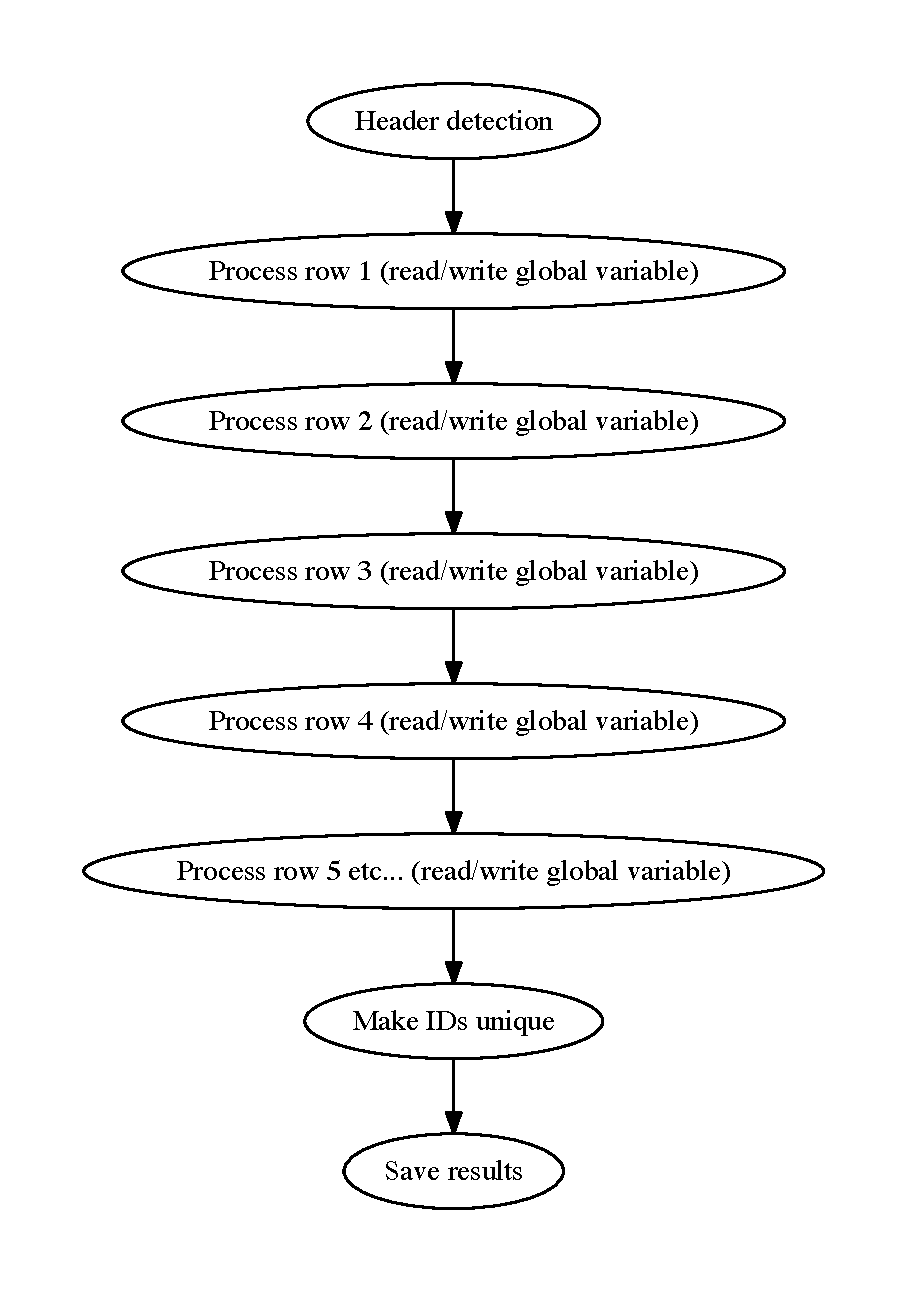
\includegraphics[width=120mm]{figures/global_variable_file_format.pdf}
  \caption[Task DAG for a file format that contains global or state variables.]{An example of a task DAG for a file format that contains global or state variables. Since each row may read and
  write the global (or state) variable, every task depends on the previous task.}
  \label{fig:global_dag}
\end{figure}

\section{Filter families}
With the help of the findings from the previous sections, families of filters with different characteristics can be identified.

\begin{itemize}
\item \textbf{Embarrassingly parallel filters} --
The filters that do not affect parallelization in any way are:
\textit{Dataset translation}, \textit{Null translation}, \textit{Relation currency},
\textit{Third party automapper}, \textit{Set value}, \textit{RegExp extract}, \textit{RegExp replace},
\textit{Dataset information}, \textit{Tradefile information}, \textit{Temporary variable}, \textit{Logger}, \textit{Skip row}, and \textit{Conditional block}.
In addition, \textit{Mapping} is included among these filters if the make unique feature is disabled.
\item \textbf{Overhead filters} -- 
Filters that introduce parallelization overhead are: \textit{Mapping} (if the make unique feature is enabled) and \textit{Header detection}.
\item \textbf{Inherently serial filters} --
The filters that enforce serial execution of the entire transformation are: \textit{Global variable}, \textit{State variable}, and \textit{Stop processing}.
\end{itemize}

\section{File format families}
In addition to the filter families, the fact that the \textit{Header detection} filter is present in all file formats makes it possible to identify the following
file format families relevant to this thesis:

\begin{itemize}
\item \textbf{Embarrassingly parallel file formats} --
  File formats that with the exception of \textit{Header detection} contain only embarrassingly parallel filters. 
\item \textbf{Extra overhead file formats} --
  Formats that in addition to \textit{Header detection} and a number of embarrassingly parallel filters also contain \textit{Mapping} with the make unique filter enabled.
\item \textbf{Inherently serial file formats} --
  Formats that contain any of the inherently serial filters.
\end{itemize}

